\documentclass[10pt,a4paper,fleqn]{article}
\usepackage[utf8]{inputenc}
\usepackage[portuguese]{babel}
\usepackage[T1]{fontenc}
\usepackage{amsmath}
\usepackage{amsfonts}
\usepackage{amssymb}
\usepackage{graphicx}
\usepackage{setspace}

\title{Disciplina M\'{e}todos Potenciais}
\author{Vanderlei C. Oliveira Jr.}
\date{}

\doublespace

\begin{document}

\begin{center}

\begin{huge}
\emph{Anomalias Magn\'{e}ticas}
\end{huge}

\bigskip
\bigskip

\begin{large}
\emph{Disciplina M\'{e}todos Potenciais}
\end{large}

\end{center}

\bigskip
\bigskip

\begin{center}

\fbox{\begin{minipage}{15em}

\begin{center}

Vanderlei C. Oliveira Jr.

Observat\'{o}rio Nacional - MCTI

Rio de Janeiro - 2015

\end{center}

\end{minipage}}

\end{center}

\clearpage

\tableofcontents

\clearpage

%%%%%%%%%%%% Anomalia de Campo Total%%%%%%%%%%%%%%
%%%%%%%%%%%%%%%%%%%%%%%%%%%%%%%%%%%%%%%%%%%%%%%%%%
\section{Anomalia de Campo Total}

\subsection{Definiç\~{a}o}

Considere uma \'{a}rea de estudo sobre uma pequena região na superfície do planeta. 
Em um dado intervalo curto de tempo, podemos considerar que a parcela do campo 
geomagnético que é produzida pelo n\'{u}cleo da Terra é 
um vetor constante em toda a \'{a}rea de estudo. Este vetor pode ser escrito como
\begin{equation}
\mathbf{F} = \| \mathbf{F} \| \, \hat{\mathbf{F}} \; ,
\label{eq:campo-geomagnetico}
\end{equation}
em que $\| \mathbf{F} \|$ é a intensidade de $\mathbf{F}$ e $\hat{\mathbf{F}}$ é um vetor unitário
dado por
\begin{equation}
\hat{\mathbf{F}} = \left[
\begin{array}{c}
cos(I) \, cos(D) \\
cos(I) \, sen(D) \\
sen(I)
\end{array}
\right] \; ,
\label{eq:versor-campo-geomagnetico}
\end{equation}
sendo $D$ e $I$ a declinação e a inclinação de $\mathbf{F}$, respectivamente, de 
acordo com a Figura \ref{fig:fig1}.

%Figuras ==>
\begin{figure}[h]
    \centering
    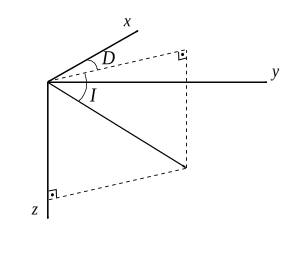
\includegraphics[scale=1]{Figs/Fig1.png}
    \caption{Representação esquemática de um vetor com declinação $D$ e inclinação $I$ referidas
        a um sistema de coordenadas Cartesianas com o eixo $x$ apontando para o norte geográfico,
        $y$ apontando para o leste e $z$ para baixo.}   
    \label{fig:fig1}
\end{figure}
%<== Figuras

A anomalia de campo total em uma determinada posição $(x_{i}, y_{i}, z_{i})$, $i = 1,...,N$,
da \'{a}rea de estudo é definida da seguinte forma:
\begin{equation}
\Delta T_{i} = \| \mathbf{F} + \mathbf{B}_{i} \| - \| \mathbf{F} \| \; ,
\label{eq:act-exata}
\end{equation}
em que $\mathbf{B}_{i}$ é a indução magn\'{e}tica produzida na posição $(x_{i}, y_{i}, z_{i})$
por corpos geol\'{o}gicos magnetizados em subsuperf\'{i}cie. Em geral, a seguinte relaç\~{a}o
\'{e} v\'{a}lida:
\begin{equation}
\| \mathbf{F} \| \gg \| \mathbf{B}_{i} \| \; , \; i = 1,...,N.
\label{eq:f-maior-maior-b}
\end{equation}
Esta relaç\~{a}o possibilita aproximar a anomalia de campo total $\Delta T_{i}$ 
(Eq. \ref{eq:act-exata}) por uma s\'{e}rie de Taylor, tal como será descrito a seguir.

\subsection{Anomalia de Campo Total aproximada}

Seja $f(\mathbf{p})$ uma funç\~{a}o escalar dada por:
\begin{equation}
\begin{split}
f(\mathbf{p}) & = \| \mathbf{p} \| \\
              & = \sqrt{\mathbf{p}^{\intercal} \mathbf{p}} \\
              & = p_{x}^{2} + p_{y}^{2} + p_{z}^{2} \; ,
\end{split}
\label{eq:funcao-norma-Euclidiana}
\end{equation}
em que $\mathbf{p}$ é um vetor dado por
\begin{equation}
\mathbf{p} = 
\left[
\begin{array}{c}
p_{x} \\
p_{y} \\
p_{z}
\end{array}
\right]_{3 \times 1} \; .
\label{eq:vetor-p}
\end{equation}
A funç\~{a}o $f(\mathbf{p})$ (Eq. \ref{eq:funcao-norma-Euclidiana}) representa a norma Euclidiana 
do vetor $\mathbf{p}$ (Eq. \ref{eq:vetor-p}), cujas componentes Cartesianas são $p_{x}$, 
$p_{y}$ e $p_{z}$. A funç\~{a}o pode ser expandida em torno de um ponto $\mathbf{p}_{0}$ 
por meio de uma s\'{e}rie de Taylor at\'{e} ordem 1 da seguinte forma:
\begin{equation}
f(\mathbf{p}_{0} + \Delta\mathbf{p}) \approx
f(\mathbf{p}_{0}) + 
\nabla f(\mathbf{p}_{0})^{\intercal} \Delta\mathbf{p} \; ,
\label{eq:funcao-f-Taylor}
\end{equation}
em que $\Delta\mathbf{p}$ é um vetor que representa uma pequena perturbaç\~{a}o
em torno de $\mathbf{p}_{0}$ $\--$ isto \'{e}, $\| \mathbf{p}_{0} \| \gg \| 
\Delta \mathbf{p} \|$ $\--$
e $\nabla f(\mathbf{p}_{0})$ \'{e} o vetor gradiente
de $f(\mathbf{p}_{0})$, que \'{e} definido como:
\begin{equation}
\nabla f(\mathbf{p}_{0}) =
\left[
\begin{array}{c}
\frac{\partial f(\mathbf{p}_{0})}{\partial p_{x}} \\
\frac{\partial f(\mathbf{p}_{0})}{\partial p_{y}} \\
\frac{\partial f(\mathbf{p}_{0})}{\partial p_{z}}
\end{array}
\right]_{3 \times 1} \; .
\label{eq:gradiente-f}
\end{equation}
Se derivarmos a Equaç\~{a}o \ref{eq:funcao-norma-Euclidiana} em relaç\~{a}o \`{a}s vari\'{a}veis
$p_{x}$, $p_{y}$ e $p_{z}$, podemos reescrever o vetor $\nabla f(\mathbf{p}_{0})$ da seguinte 
forma:
\begin{equation}
\begin{split}
\nabla f(\mathbf{p}_{0}) & = 
\dfrac{\mathbf{p}_{0}}{\sqrt{\mathbf{p}_{0}^{\intercal} \mathbf{p}_{0}}} \\
                         & = \hat{\mathbf{p}}_{0} \; ,
\end{split}
\label{eq:gradiente-f-2}
\end{equation}
sendo $\hat{\mathbf{p}}_{0}$ um vetor unit\'{a}rio com a mesma direç\~{a}o e sentido
do vetor $\mathbf{p}_{0}$. Substituindo esta express\~{a}o (Eq. \ref{eq:gradiente-f-2})
na Equaç\~{a}o \ref{eq:funcao-f-Taylor} temos que:
\begin{equation}
f(\mathbf{p}_{0} + \Delta\mathbf{p}) \approx
\| \mathbf{p}_{0} \| + 
\hat{\mathbf{p}}_{0}^{\intercal} \Delta\mathbf{p} \; .
\label{eq:funcao-f-Taylor-2}
\end{equation}
Utilizando esta aproximaç\~{a}o por s\'{e}rie de Taylor (Eq. \ref{eq:funcao-f-Taylor-2})
e considerando que a induç\~{a}o magn\'{e}tica $\mathbf{B}_{i}$, $i=1,...,N$ (Eq. 
\ref{eq:act-exata}) \'{e} uma pequena perturbaç\~{a} no campo geomagn\'{e}tico 
$\mathbf{F}$ (Eq. \ref{eq:campo-geomagnetico}), $\--$ ou seja, que a Equaç\~{a}o
\ref{eq:f-maior-maior-b} \'{e} v\'{a}lida $\--$ podemos aproximar a anomalia de campo
total $\Delta T_{i}$ (Eq. \ref{eq:act-exata}) pela seguinte express\~{a}o:
\begin{equation}
\begin{split}
\Delta T_{i}^{a} & = \| \mathbf{F}\| + \dfrac{\mathbf{F}^{\intercal}}
                     {\sqrt{\mathbf{F}^{\intercal} \mathbf{F}}} 
                     \mathbf{B}_{i} - \| \mathbf{F} \| \\
                 & = \hat{\mathbf{F}}^{\intercal} \mathbf{B}_{i} \; ,
\end{split}
\label{eq:act-aprox}
\end{equation}
em que $\hat{\mathbf{F}}$ é um vetor unit\'{a}rio com a mesma direç\~{a}o e sentido
do campo geomagn\'{e}tico $\mathbf{F}$ (Eq. \ref{eq:campo-geomagnetico}). Vale
ressaltar que esta aproximaç\~{a}o (Eq. \ref{eq:act-aprox}) da anomalia de campo 
total (Eq. \ref{eq:act-exata}) pressup\~{o}e a validade da relaç\~{a}o descrita pela
Equaç\~{a}o \ref{eq:f-maior-maior-b}. 

\begin{flushleft}
\dotfill
\end{flushleft}

\subsubsection{Exerc\'{i}cio}

Seja $\mathbf{B}$ um vetor $3 \times 1$ que representa a induç\~{a}o magn\'{e}tica produzida
por um corpo geol\'{o}gico em uma determinada posiç\~{a}o na superf\'{i}cie da Terra. Este
vetor pode ser escrito como:
\begin{equation}
\mathbf{B} = \| \mathbf{B} \| \, \hat{\mathbf{B}} \; ,
\label{eq:ex321-vetor-b}
\end{equation}
em que $\| \mathbf{B} \|$ \'{e} a intensidade de $\mathbf{B}$ e $\hat{\mathbf{B}}$ é um vetor unitário
dado por
\begin{equation}
\hat{\mathbf{B}} = \left[
\begin{array}{c}
cos(i) \, cos(d) \\
cos(i) \, sen(d) \\
sen(i)
\end{array}
\right] \; ,
\label{eq:ex321-versor-b}
\end{equation}
sendo $d$ e $i$ a declinação e a inclinação de $\mathbf{B}$, respectivamente, de 
acordo com a Figura \ref{fig:fig3}. Utilizando este vetor $\mathbf{B}$ (Eq. 
\ref{eq:ex321-vetor-b}) e um vetor $\mathbf{F}$ que descreva o campo geomagn\'{e}tico
\'{e} poss\'{i}vel calcular a anomalia de campo total $\Delta T$ (Eq. 
\ref{eq:act-exata}) e a anomalia de campo total aproximada $\Delta T^{a}$ (Eq. 
\ref{eq:act-aprox}). \'{E} de se esperar que, quanto maior a intensidade de $\mathbf{F}$,
menos deve ser a diferença entre  $\Delta T$ (Eq. \ref{eq:act-exata}) e $\Delta T^{a}$ 
(Eq. \ref{eq:act-aprox}). Sendo assim:

\begin{enumerate}

\item Defina valores para $\| \mathbf{B} \|$, $d$ e $i$ (Eqs. \ref{eq:ex321-vetor-b} 
      e \ref{eq:ex321-versor-b}) e calcule um vetor $\mathbf{B}$.

\item Defina valores para $D$ e $I$ (Eq. \ref{eq:versor-campo-geomagnetico}) e calcule
      um vetor unit\'{a}rio $\hat{\mathbf{F}}$.

\item Defina um conjunto de $N$ valores $F = \| \mathbf{F} \|$.
      Estes valores devem formar uma s\'{e}rie crescente, que começa com valores menores
      que $\| \mathbf{B} \|$ (definido no item 1) e terminam com valores muito maiores
      que $\| \mathbf{B} \|$ (definido no item 1).
      
\item Utilizando o vetor unit\'{a}rio $\hat{\mathbf{F}}$ definido no item 2 e cada um 
      dos $N$ valores $F$ definidos no item anterior, calcule um vetor $\mathbf{F}$.
      
\item Para cada um dos $N$ vetores $\mathbf{F}$ definidos no item anterior, calcule a
      anomalia de campo total $\Delta T$ (Eq. \ref{eq:act-exata}) e a anomalia de campo 
      total aproximada $\Delta T^{a}$ (Eq. \ref{eq:act-aprox}).
      
\item Faça um gr\'{a}fico da anomalia de campo total predita pelas Equaç\~{o}es \ref{eq:act-exata}
      e \ref{eq:act-aprox} em funç\~{a}o da razão $F/\| \mathbf{B} \|$.

\item A partir de qual valor $F/\| \mathbf{B} \|$ a diferença entre os valores preditos
      pelas Equaç\~{o}es \ref{eq:act-exata} e \ref{eq:act-aprox} é m\'{i}nima?

\end{enumerate}


\begin{flushleft}
\dotfill
\end{flushleft}

\bigskip
\bigskip

\end{document}
